\section{设计方案}
\subsection{总体设计思路}

本设计基于实验 4 的简单 5 级流水线设计,在扩展至 57 条指令后,将 CPU 封装成 SRAM 接口,并依照图\ref{fig:AXI},将 CPU (SRAM MIPS) 封装将成类 SRAM 接口,添加 I Cache 和 D Cache,通过龙芯杯提供的转接桥和 AXI 接口转换模块将系统封装成 AXI 接口。根据实验文档中介绍的 MIPS 内存布局,通过 Bridge1x2 和 Bridge2x1 将访问数据存储器的路径分为经过 D Cache 和不经过 D Cache 的两条线路。

\begin{figure}[htbp]
    \centering
    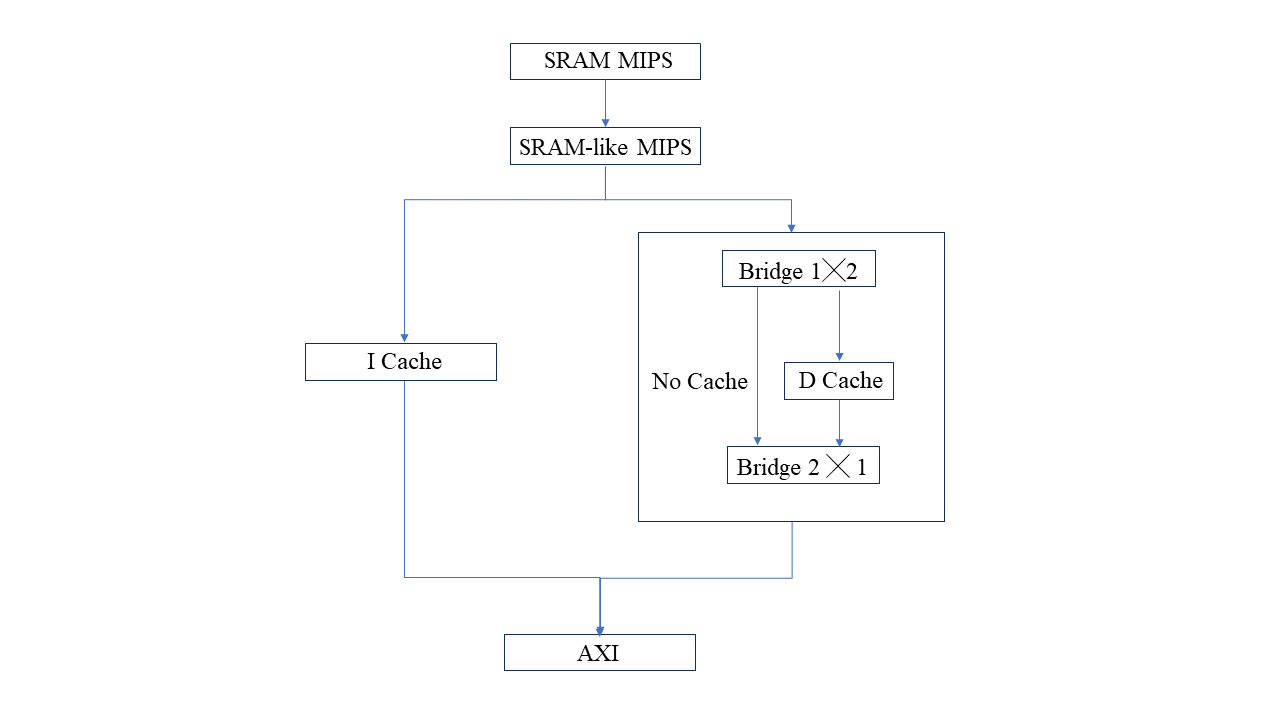
\includegraphics[width=0.8\textwidth]{image/axi.PNG}
    \caption{ AXI 接口转换}
    \label{fig:AXI}
\end{figure}

D Cache 使用多路组相联 LRU 替换策略的写回 cache,\ref{fig:cache}展示本设计中 cache 的三个状态,空闲、读内存、写内存。写直达(Write through)虽然具有强一致性保证,但是效率低,故采用写回策略。在进行块的覆盖时,如果待覆盖的块 dirty 位为 1,则需要执行写回操作。采用 LRU 替换策略,能满足程序局部性要求且有较高命中率。

\begin{figure}[htbp]
    \centering
    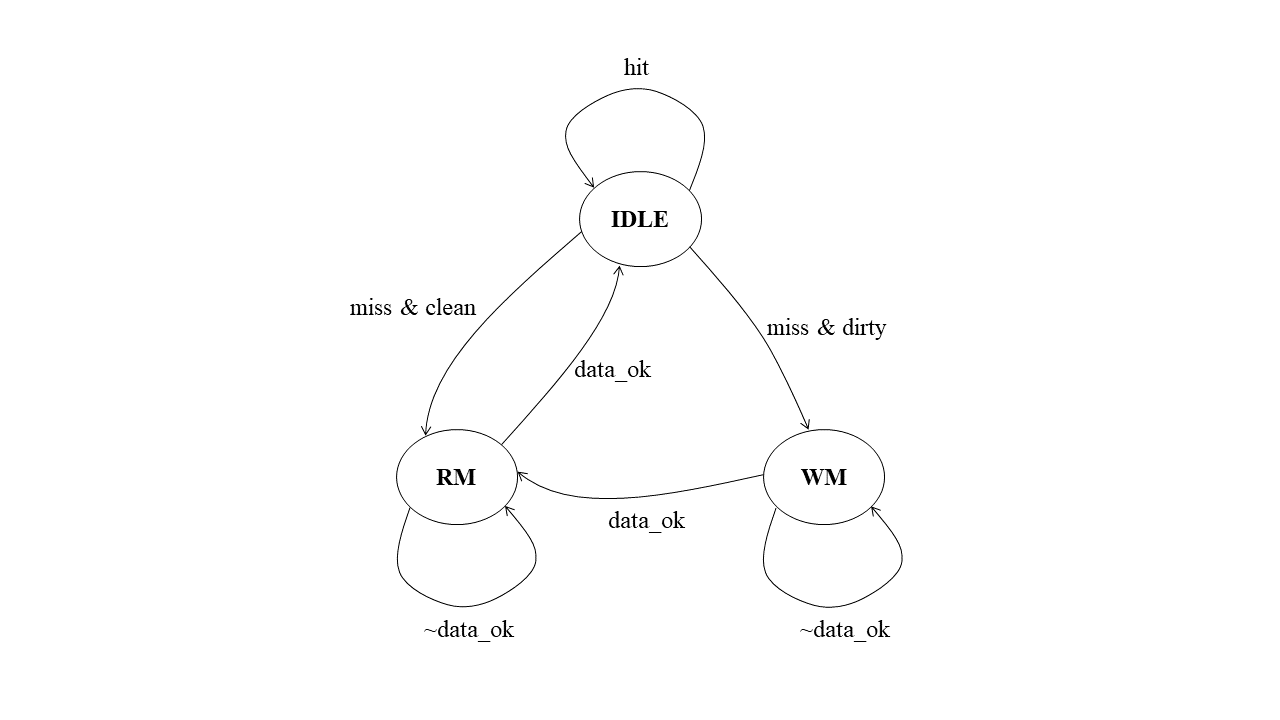
\includegraphics[width=0.8\textwidth]{image/statetrans.PNG}
    \caption{cache有限状态机}
    \label{fig:cache}
\end{figure}

基于实验 4 实现的五级流水线 CPU,通过添加和修改 CPU 内部逻辑,主要包括 controller、 datapath、 ALU、 HILO 寄存器,将 10 条指令扩展到 52 条指令,通过添加 CP0、调整数据通路和控制信号,并添加异常处理模块实现 5 条内陷和特权指令。图\ref{fig:datapath}展示本设计的数据通路(忽略 controller 和 hazard 模块中的细节,仅标注由 controller 输出的信号)。

\begin{figure}[H]
    \centering
    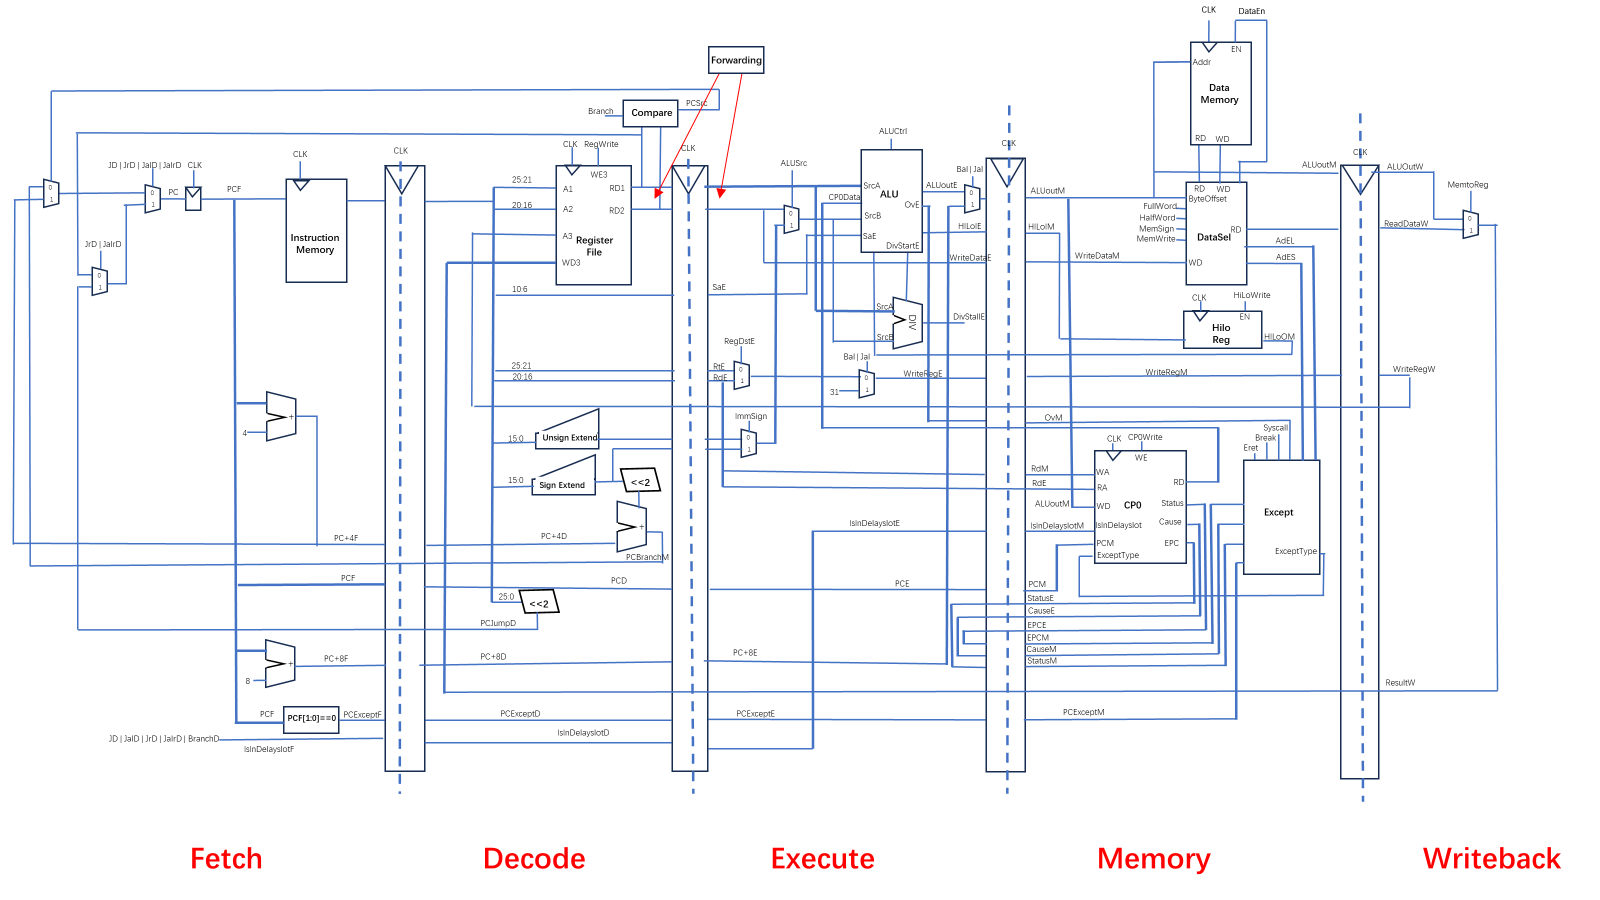
\includegraphics[width=1\linewidth]{image/datapath.png}
    \caption{数据通路}
    \label{fig:datapath}
\end{figure}

设计的流程包括以下 5 步:

\begin{itemize}
    \item 基于实验 4 的 CPU,按指令的类别完成各类指令的添加,并分别完成功能测试。
    \item 将 CPU 封装成 SRAM 接口,并进行 SRAM 接口的功能测试。
    \item 将 CPU 封装将成类 SRAM 接口并转换为 AXI 接口,并进行 AXI 接口的功能测试。
    \item 为实现了 AXI 接口的 CPU 添加 cache,并进行性能测试和上板测试。
    \item 优化原有的 write-through 直接映射 cache 为组相联写回 cache,尝试提升性能测试得分。
\end{itemize}

\subsubsection{扩展指令设计思路}
根据《指令及对应机器码\_2018》和《“系统能力培养大赛”MIPS指令系统规范\_v1.01》,待添加指令如下:
\begin{itemize}
 \item 逻辑运算指令:and,or,xor,nor,andi,ori,xori,lui
 \item 移位指令:sll,srl,sra,sllv,srlv,srav
 \item 数据移动指令:mfhi,mflo,mthi,mtlo
 \item 算数运算指令:add,addu,sub,subu,slt,sltu,mult,multu,div,divu,addi,addiu,slti,sltiu
 \item 分支跳转指令:jr,jalr,j,jal,beq,bgtz,blez,bne,bltz,bltzal,bgez,bgezal
 \item 访存指令:lb,lbu,lh,lhu,lw,sb,sh,sw
 \item 自陷指令:break,syscall
 \item 特权指令:mtc0,mfc0,eret
\end{itemize}

下发的资料为每一类指令提供了测试文件(.coe 文件),为封装成 SRAM 接口和 AXI 接口的系统提供了功能测试文件,为 AXI 接口提供了性能测试文件。将测试文件导入 inst\_ram,确认 trace 文件一致后,进行仿真,观察控制台输出结果与仿真波形图确认实现是否正确。

\begin{figure}[htbp]
    \centering
    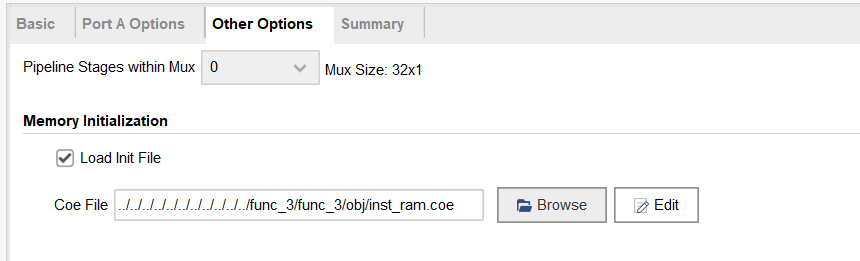
\includegraphics[width=0.8\textwidth]{image/coe.png}
    \caption{添加coe文件}
    \label{fig:my_label}
\end{figure}

对于各信号的命名,本设计根据其功能含义进行简写,尽可能遵循教材\cite{computer-organization-and-design}的命名风格,采用驼峰命名法,并在其后附加相应的字母(F、D、E、M、W)以标识信号所在的流水级,datapath 中除clock 和 reset 信号外,全部标明了流水级,便于调试。

对于逻辑运算指令,基本可复用实验 4 原有数据通路(需添加无符号立即数扩展模块和对应的控制信号),针对每种指令设置 aluctrl 信号,并在 ALU 中完成对于的运算。

对于移位指令,需将 sa 字段传递至 ALU,则可像逻辑运算指令一样完成运算。

对于数据移动指令,本设计中 HILO 寄存器在 EX 阶段读数据、在 MEM 阶段写数据。通过复用 ALU 相关数据通路,使 ALU 和 HILO 寄存器之间形成环路,从而简化了设计复杂度。

对于算数运算指令,除除法指令需要进行特殊处理外,其余指令可直接复用已有的数据通路。后文将对本设计中的除法器作更详细介绍。

对于分支跳转指令,需扩展 PCSrcD 信号的实现,并为跳转链接添加额外的数据通路和控制信号。后文将对分支跳转指令的实现作详细介绍。

对于访存指令,需要扩展内存读写相关逻辑。读数据和写数据仍以 32 位为单位进行,但需要调整数据存储器的写使能信号,或从读出的数据选择所需要的部分。考虑到该部分于数据存储器交互的性质,同时为了尽可能减少对数据通路的修改,本设计中使用位于数据通路外的 DataSel 模块完成访存功能。

对于自陷指令、特权指令和异常处理,本设计采用实验文档推荐的方式使 CP0 在 EX 阶段读数据、在 MEM 阶段写数据。这与 HILO 寄存器的设计非常相似。

\newpage
\subsection{模块设计}
% \textcolor{red}{对模块内部设计方案进行更进一步描述。可以包含:模块的功能意图,模块的输入输出,模块内部的数据通路和控制逻辑,以及可能的软硬件交互机制。分类介绍指令扩展}

\subsubsection{分支跳转指令实现设计}

本设计共实现了 12 条转移指令,其中 BEQ、J 指令在实验四中已经实现,BNE、 BGEZ、 BGTZ、 BLEZ、BLTZ 功能和 BEQ 类似,只需要对跳转控制信号的产生进行扩展——在 ID 阶段将判断相等的逻辑替换成 compare 模块,其余部分复用 BEQ 指令的数据通路即可。JR 指令无条件跳转到寄存器 rs 保存的目标地址,只需新增 SrcAD(进行相关的数据前推后的 rs 寄存器值)连到 nextPCF 的多选器。JAL 指令除无条件跳转外,还要将 PC + 8 写入 31 号寄存器中。本设计没有复用 ALU 的数据通路,而是类比 PC + 4,直接计算 PC + 8 并通过多选器判断写寄存器的值。BLTZAL 和 BGEZAL 指令类似于 BEQ 和 JAL 指令,只需要产生相应的控制信号而不需要对数据通路进行修改。

\begin{table}[h]
\centering
\begin{tabular}{|c|c|c|c|}
\hline
\textbf{信号名}  & \textbf{位宽} & \textbf{功能描述}\\ \hline 
ForwardAD & 1 & Forwarding signal for operand A in the ID stage \\ \hline
ForwardBD & 1 & Forwarding signal for operand B in the ID stage \\ \hline
NextPCF & 32 & Next PC in F stage \\ \hline
PCPlus4F & 32 & PC + 4 in F stage which used for no branch \\ \hline
PCPlus8F &32 & PC + 8 in F stage which used for Jal like instructions \\ \hline
PCJumpD & 32 & Destination address of jump \\ \hline
PCBrachD & 32 & Destination address of branch \\ \hline
SrcAD & 32 & Value of rd1 after forwarding, used for comparing \\ \hline
SrcBD & 32 & Value of rd2 after forwarding, used for comparing \\ \hline
\end{tabular}
\caption{分支跳转主要信号和变量}
\label{分支跳转主要信号和变量}
\end{table}

分支指令在 ID 阶段读寄存器的数据通路见图\ref{fig:brach}.
\begin{figure}[htbp]
    \centering
    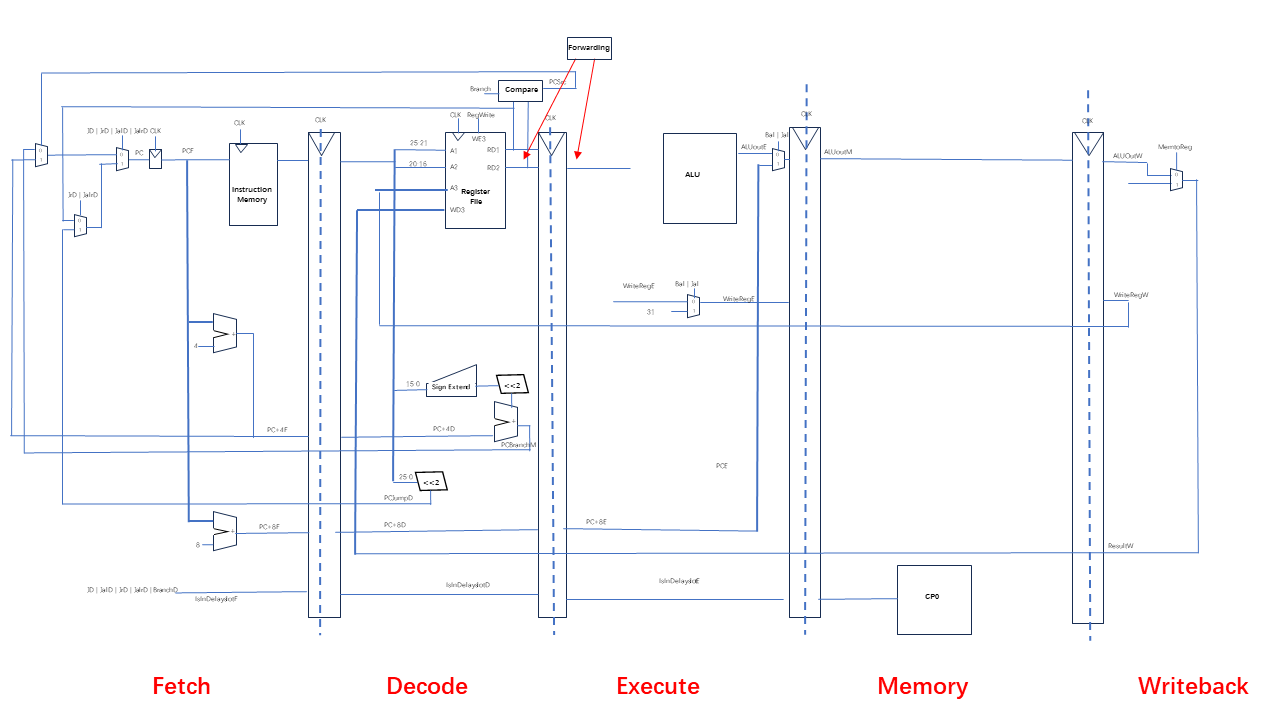
\includegraphics[width=0.8\textwidth]{image/branch.PNG}
    \caption{分支跳转指令设计通路图}
    \label{fig:brach}
\end{figure}

分支跳转指令、延迟槽的控制信号相关代码如下。

\begin{lstlisting}[language=Verilog]
//If jump: next PC is jump address
//If branch: next PC is branch address
//Else next PC is PC + 4
assign NextPCF =
    ((JD | JrD | JalD | JalrD) == 1'h1) ?  PCJumpD :
    (PCSrcD == 1'h1) ? PCBranchD : PCPlus4F;
assign PCPlus4F = PCF + 32'h4;
//For bal and jal: save return address PC + 8.
assign PCPlus8F = PCF + 32'h8;
assign PCExceptF = PCF[1:0] == 2'b00 ? 1'b0 : 1'b1;
//Refer to `https://co.ccslab.cn/basic/extend_57/#_7`:
assign IsInDelaySlotF = JD | JalD | JrD | JalrD | BranchD;
assign SrcAD = (ForwardAD == 1'h1 ? ALUOutM : rd1D);
assign SrcBD = (ForwardBD == 1'h1 ? ALUOutM : rd2D);
//Branch address
assign PCBranchD = { SignImmD[29:0], 2'b00 } + PCPlus4D;
//If jr or jalr: jump address is from register rs
//If j or jal: jump address is from instruction
assign PCJumpD = ((JrD | JalrD) == 1'b1) ? SrcAD : { PCPlus4D[31:28], InstrD[25:0], 2'h0 };
\end{lstlisting}

\subsubsection{除法器}

本项目采用基础的恢复余数除法器\cite{computer-organization-and-design}。

对于 DIV 指令,将首先计算操作数绝对值的余数和商,再根据操作数的符号判断余数和商的符号。因此需要重点考虑 DIVU 指令。

图\ref{fig:除法器结构}展示了一个基础的除法器的结构。

\begin{figure}[H]
    \centering
    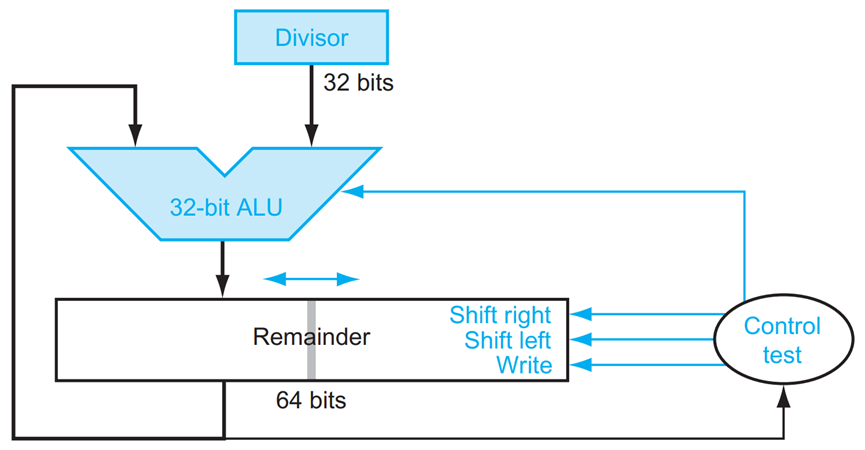
\includegraphics[width=1\linewidth]{image/除法器结构.png}
    \caption{除法器结构示意图}
    \label{fig:除法器结构}
\end{figure}

无符号除法计算流程如图\ref{fig:除法器流程图}所示。

\begin{figure}
    \centering
    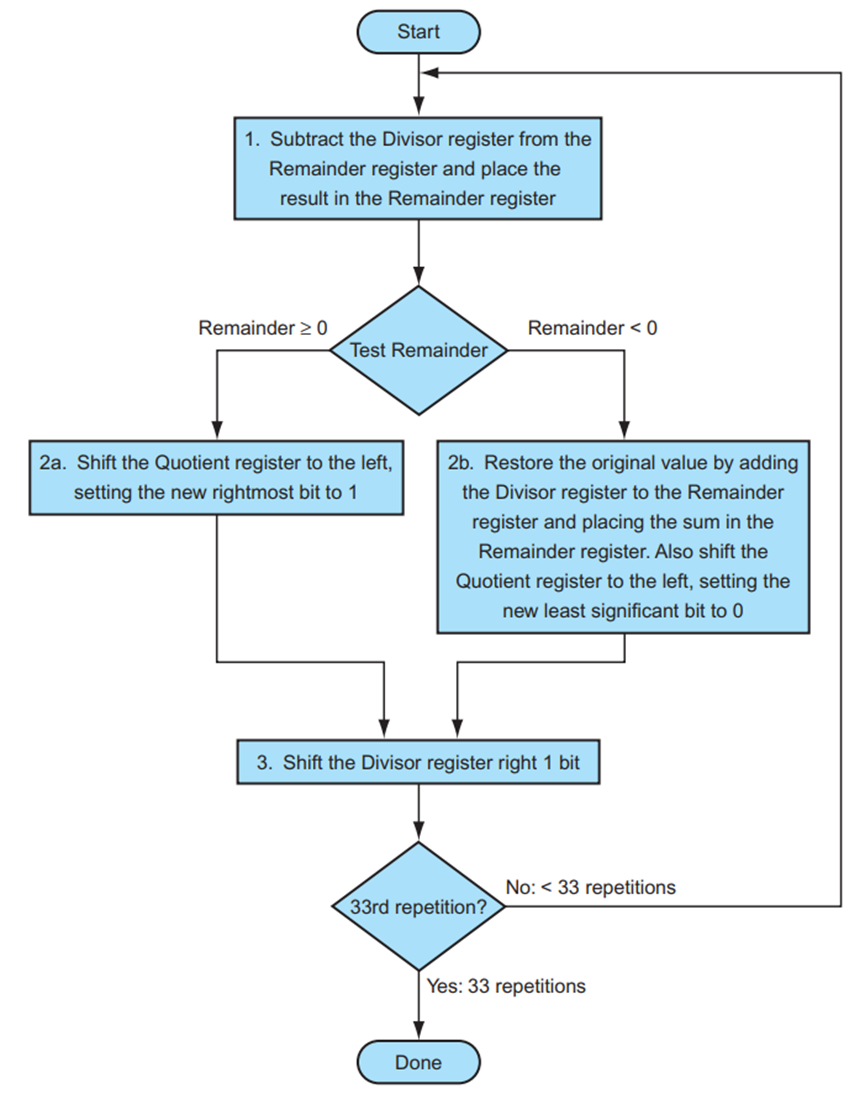
\includegraphics[width=1\linewidth]{image/除法器流程图.png}
    \caption{除法器流程图}
    \label{fig:除法器流程图}
\end{figure}

除法器的接口如表\ref{除法器接口}所示。

\begin{table}[h]
\centering
\begin{tabular}{|c|c|c|c|}
\hline
\textbf{信号名}  & \textbf{位宽} & \textbf{功能描述}\\ \hline 
clock &  1 & 时钟信号 \\ \hline
reset & 1 & 复位信号 \\ \hline
SrcA & 32 & 被除数 \\ \hline
SrcB & 32 & 除数 \\ \hline
start & 1 & 除法运算开始信号;start 为 1 表示正在进行除法运算 \\ \hline
is\_signed & 1 & 区分有符号除法和无符号除法;is\_signed 为 1 表示进行有符号除法运算 \\ \hline
stall &  1 & 除法阻塞信号;进行除法运算时需阻塞流水线 \\ \hline
result & 64 & 除法运算的结果;高 32 位为余数、低 32 位为商 \\ \hline
\end{tabular}
\caption{除法器接口}
\label{除法器接口}
\end{table}

相关代码如下。

\begin{lstlisting}
// 试商:余数 = 余数 - 除数
// 如果结果小于 0(CO 为 0)则恢复余数
// AbsRemainder 为试商前的余数
// sub_result 为更新后的余数
assign { CO, sub_result } = { 1'b0, AbsRemainder } + NegSrcB;
assign mux_result = CO ? sub_result : { 1'b0, AbsRemainder };
assign result = { Remainder, Quotient };
assign stall = |cnt;

always @ (posedge clock, posedge reset) begin
    if (reset) begin
        cnt <= 0;
        start_cnt <= 0;
    end else if (!start_cnt & start) begin
        cnt <= 1;
        start_cnt <= 1;
        SrcASave <= SrcA;
        SrcBSave <= SrcB;
        SR <= { 31'b0, AbsSrcA, 1'b0 };
        NegSrcB <= (is_signed & SrcB[31]) ? { 1'b1, SrcB } : ~{ 1'b0, SrcB } + 1'b1;
    end else if(start_cnt) begin
        if (cnt == 32) begin
            cnt <= 0;
            start_cnt <= 0;
            SR[63:32] <= mux_result[31:0];
            SR[0] <= CO;
        end else begin
            cnt <= cnt + 1;
            // 置位并左移
            SR[63:0] <= { mux_result[30:0], SR[31:1], CO, 1'b0 };
        end
    end
end
\end{lstlisting}

\subsubsection{hazard}

HILO 寄存器主要用于保存乘法指令和除法指令的计算结果,因此需要将 ALU 的计算结果传递至 HILO 寄存器;还需要从 HILO 寄存器中读出数据到寄存器堆。

本设计中复用了逻辑运算、算术运算指令通过 ALU 完成计算并将计算结果写入寄存器堆的数据通路逻辑,将 HILO 寄存器的输出传入 ALU,进而能够将数据写入寄存器堆。由此,HILO 寄存器与 ALU 之间形成一个简单的环路。通过将 HILO 寄存器的时钟信号取反的方式避免额外的数据前推,简化了数据通路,但增大了系统延迟。

各级流水线的阻塞和刷新信号如下。

\begin{lstlisting}[language=Verilog]
assign StallF = lwstall | branchstall | jrstall | stall_all;
assign StallD = StallF;
assign StallE = stall_all;
assign StallM = stall_all;
assign StallW = stall_all;

assign FlushF = FlushExcept & ~stall_all;
assign FlushD = FlushExcept & ~stall_all;
assign FlushE = (lwstall | branchstall | JD | JrD | FlushExcept) & ~stall_all;
assign FlushM = FlushExcept & ~stall_all;
assign FlushW = FlushExcept & ~stall_all;
\end{lstlisting}

其中 stall\_all 表示对流水线阻塞多个时钟周期的信号。

\begin{lstlisting}[language=Verilog]
assign stall_all = i_stall | d_stall | DivStallE;
\end{lstlisting}

\subsubsection{hilo寄存器}

HILO 寄存器主要用于保存乘法指令和除法指令的计算结果,因此需要将 ALU 的计算结果传递至 HILO 寄存器;还需要从 HILO 寄存器中读出数据到寄存器堆。

本设计中复用了逻辑运算、算术运算指令通过 ALU 完成计算并将计算结果写入寄存器堆的数据通路逻辑,将 HILO 寄存器的输出传入 ALU,进而能够将数据写入寄存器堆。由此,HILO 寄存器与 ALU 之间形成一个简单的环路。通过将 HILO 寄存器的时钟信号取反的方式避免额外的数据前推,简化了数据通路,但增大了系统延迟。

\subsubsection{cache}

在实验提供的 write-through 直接映射 cache 的基础上,参考实验文档和其他资料,设计了组相联写回 cache 的状态机,实现了采用 LRU 替换策略的 2 路组相联写回 cache 和采用 PLRU 替换策略的 4 路组相联写回 cache。

Cache 状态机实现代码如下。

\begin{lstlisting}[language=Verilog]
//FSM
parameter IDLE = 2'b00;
parameter RM = 2'b01;
parameter WM = 2'b10;
reg [1:0] state;
always @ (posedge clk) begin
    if (rst) begin
        state <= IDLE;
    end else begin
        case(state)
            IDLE:
                state <=
                    //Write back. 
                    cpu_data_req & miss & dirty ? WM :
                    //Read memory.
                    cpu_data_req & miss & clean ? RM :
                    //Hit
                    cpu_data_req & hit ? IDLE : IDLE;
            RM:
                //Wait until memory reading is finished.
                state <= cache_data_data_ok ? IDLE : RM;
            WM:
                //Wait until memory writing is finished.
                //Write memory and then read memory.
                state <= cache_data_data_ok ? RM : WM;
        endcase
    end
end
\end{lstlisting}

在访问 cache 命中时或者替换 cache 块时,需要对 cache 内容进行更新,并维护每组最近最少访问的 cache 块。相关代码如下。

\begin{lstlisting}[language=Verilog]
integer t;
always @ (negedge clk) begin
    if (rst) begin
        for (t = 0; t < CACHE_DEEPTH; t = t + 1) begin
            cache_valid_0[t] <= 0;
            cache_dirty_0[t] <= 0;
            cache_valid_1[t] <= 0;
            cache_dirty_1[t] <= 0;
            cache_LRU[t] <= 0;
        end
    end else begin
        //If read cache hit: set cache_LRU.
        //If write cache hit: update cache.
        if (cpu_data_req & hit) begin
            if (cpu_data_wr) begin
                case (hit_num)
                    0: begin
                        cache_block_0[index] <= write_cache_data;
                        cache_dirty_0[index] <= 1;
                    end
                    1: begin
                        cache_block_1[index] <= write_cache_data;
                        cache_dirty_1[index] <= 1;
                    end
                    default: ;
                endcase
            end
            cache_LRU[index] <= ~hit_num;
        end
        //If read cache miss: update cache line after reading data from memory
        if (read_req & cache_data_data_ok) begin
            case (replace_num)
                0: begin
                    cache_valid_0[index_save] <= 1'b1;
                    cache_dirty_0[index_save] <= wr_save;
                    cache_block_0[index_save] <= update_data;
                    cache_tag_0  [index_save] <= tag_save;
                end
                1: begin
                    cache_valid_1[index_save] <= 1'b1;
                    cache_dirty_1[index_save] <= wr_save;
                    cache_block_1[index_save] <= update_data;
                    cache_tag_1  [index_save] <= tag_save;
                end
                default: ;
            endcase
            cache_LRU[index_save] <= ~replace_num;
        end
    end
end
\end{lstlisting}
